% cover-createspace-quarto.tex

% make a cover PDF for CreateSpace Crown Quarto booksize.

% note: Lulu will flatten this PDF and get the colors wrong. Convert
% this PDF to PNG first (eg, using GIMP: just import at 300dpi then
% export as PNG).

\documentclass{memoir}
\usepackage[sfdefault]{universalis}
\usepackage[osf]{Baskervaldx} % oldstyle figures

\newcommand{\olpath}{../../}

\usepackage[absolute,overlay]{textpos}
\usepackage{rotating}
\usepackage[cmyk]{xcolor}

\definecolor{leadbeater}{RGB}{248,154,14}

\newlength{\coverheight}
\newlength{\coverwidth}
\newlength{\spinewidth}
\newlength{\spinepos} % spine starts here, width = \spinewidth
\newlength{\coverpos} % front cover starts here, width = \spinepos
\newlength{\sheetwidth}
\setlength{\sheetwidth}{0.002252in}

\setlength{\coverheight}{9.69in}  % trim height
\setlength{\spinepos}{7.44in} % trim width
\setlength{\spinewidth}{362\sheetwidth}

% compute actual widths
\addtolength{\coverheight}{.25in} % add bleed
\addtolength{\spinepos}{.125in} % add bleed
\setlength{\coverwidth}{\spinepos}
\addtolength{\coverwidth}{\coverwidth}
\addtolength{\coverwidth}{\spinewidth}

% \coverpos = \spinepso + \spinewidth
\setlength{\coverpos}{\spinepos}
\addtolength{\coverpos}{\spinewidth}

% set stock size to total width & height of cover 
\setstocksize{\coverheight}{\coverwidth}

% pagesize = stocksize
\settrimmedsize{\stockheight}{\stockwidth}{*}
\settrims{0pt}{0pt}

% no margins or headers
\setlrmarginsandblock{0pt}{0pt}{*}
\setheadfoot{0pt}{0pt}
\setulmarginsandblock{0pt}{0pt}{*}
\setheadfoot{0pt}{0pt}
\setlength{\headsep}{0pt}


% finalize the page layout
\checkandfixthelayout[fixed]
\typeoutlayout

\color{black}

\begin{document}
% no folios
\pagestyle{empty}

% set back background to Matt's orange

\pagecolor{leadbeater}

% make a spine
\begin{textblock*}{\spinewidth}(\spinepos,0bp)%
\noindent\hfil\rotatebox{-90}{% make spine text readable when book is lying cover up
      \hbox to \coverheight{\hfil
          \huge\sffamily\bfseries
            Sets, Logic, Computation\hfil F17\hspace{2cm}}}\hfil
\end{textblock*}
\newbox\adjust
% make front cover
\begin{textblock*}{\spinepos}(\coverpos,0pt)
  \noindent\hfil
  \begin{minipage}[b][\coverheight][s]{.8\spinepos}
   \vspace{1.5cm}
    \begin{raggedright}
      \fontsize{32pt}{34pt}\selectfont\bfseries\sffamily%
      Sets, Logic, Computation\\
      \normalfont\fontsize{18pt}{0pt}\selectfont\bfseries\itshape%
      \rule{.8\spinepos}{5pt}\\[5pt]
      An Open Logic Text
    \end{raggedright}
    \noindent\vskip2cm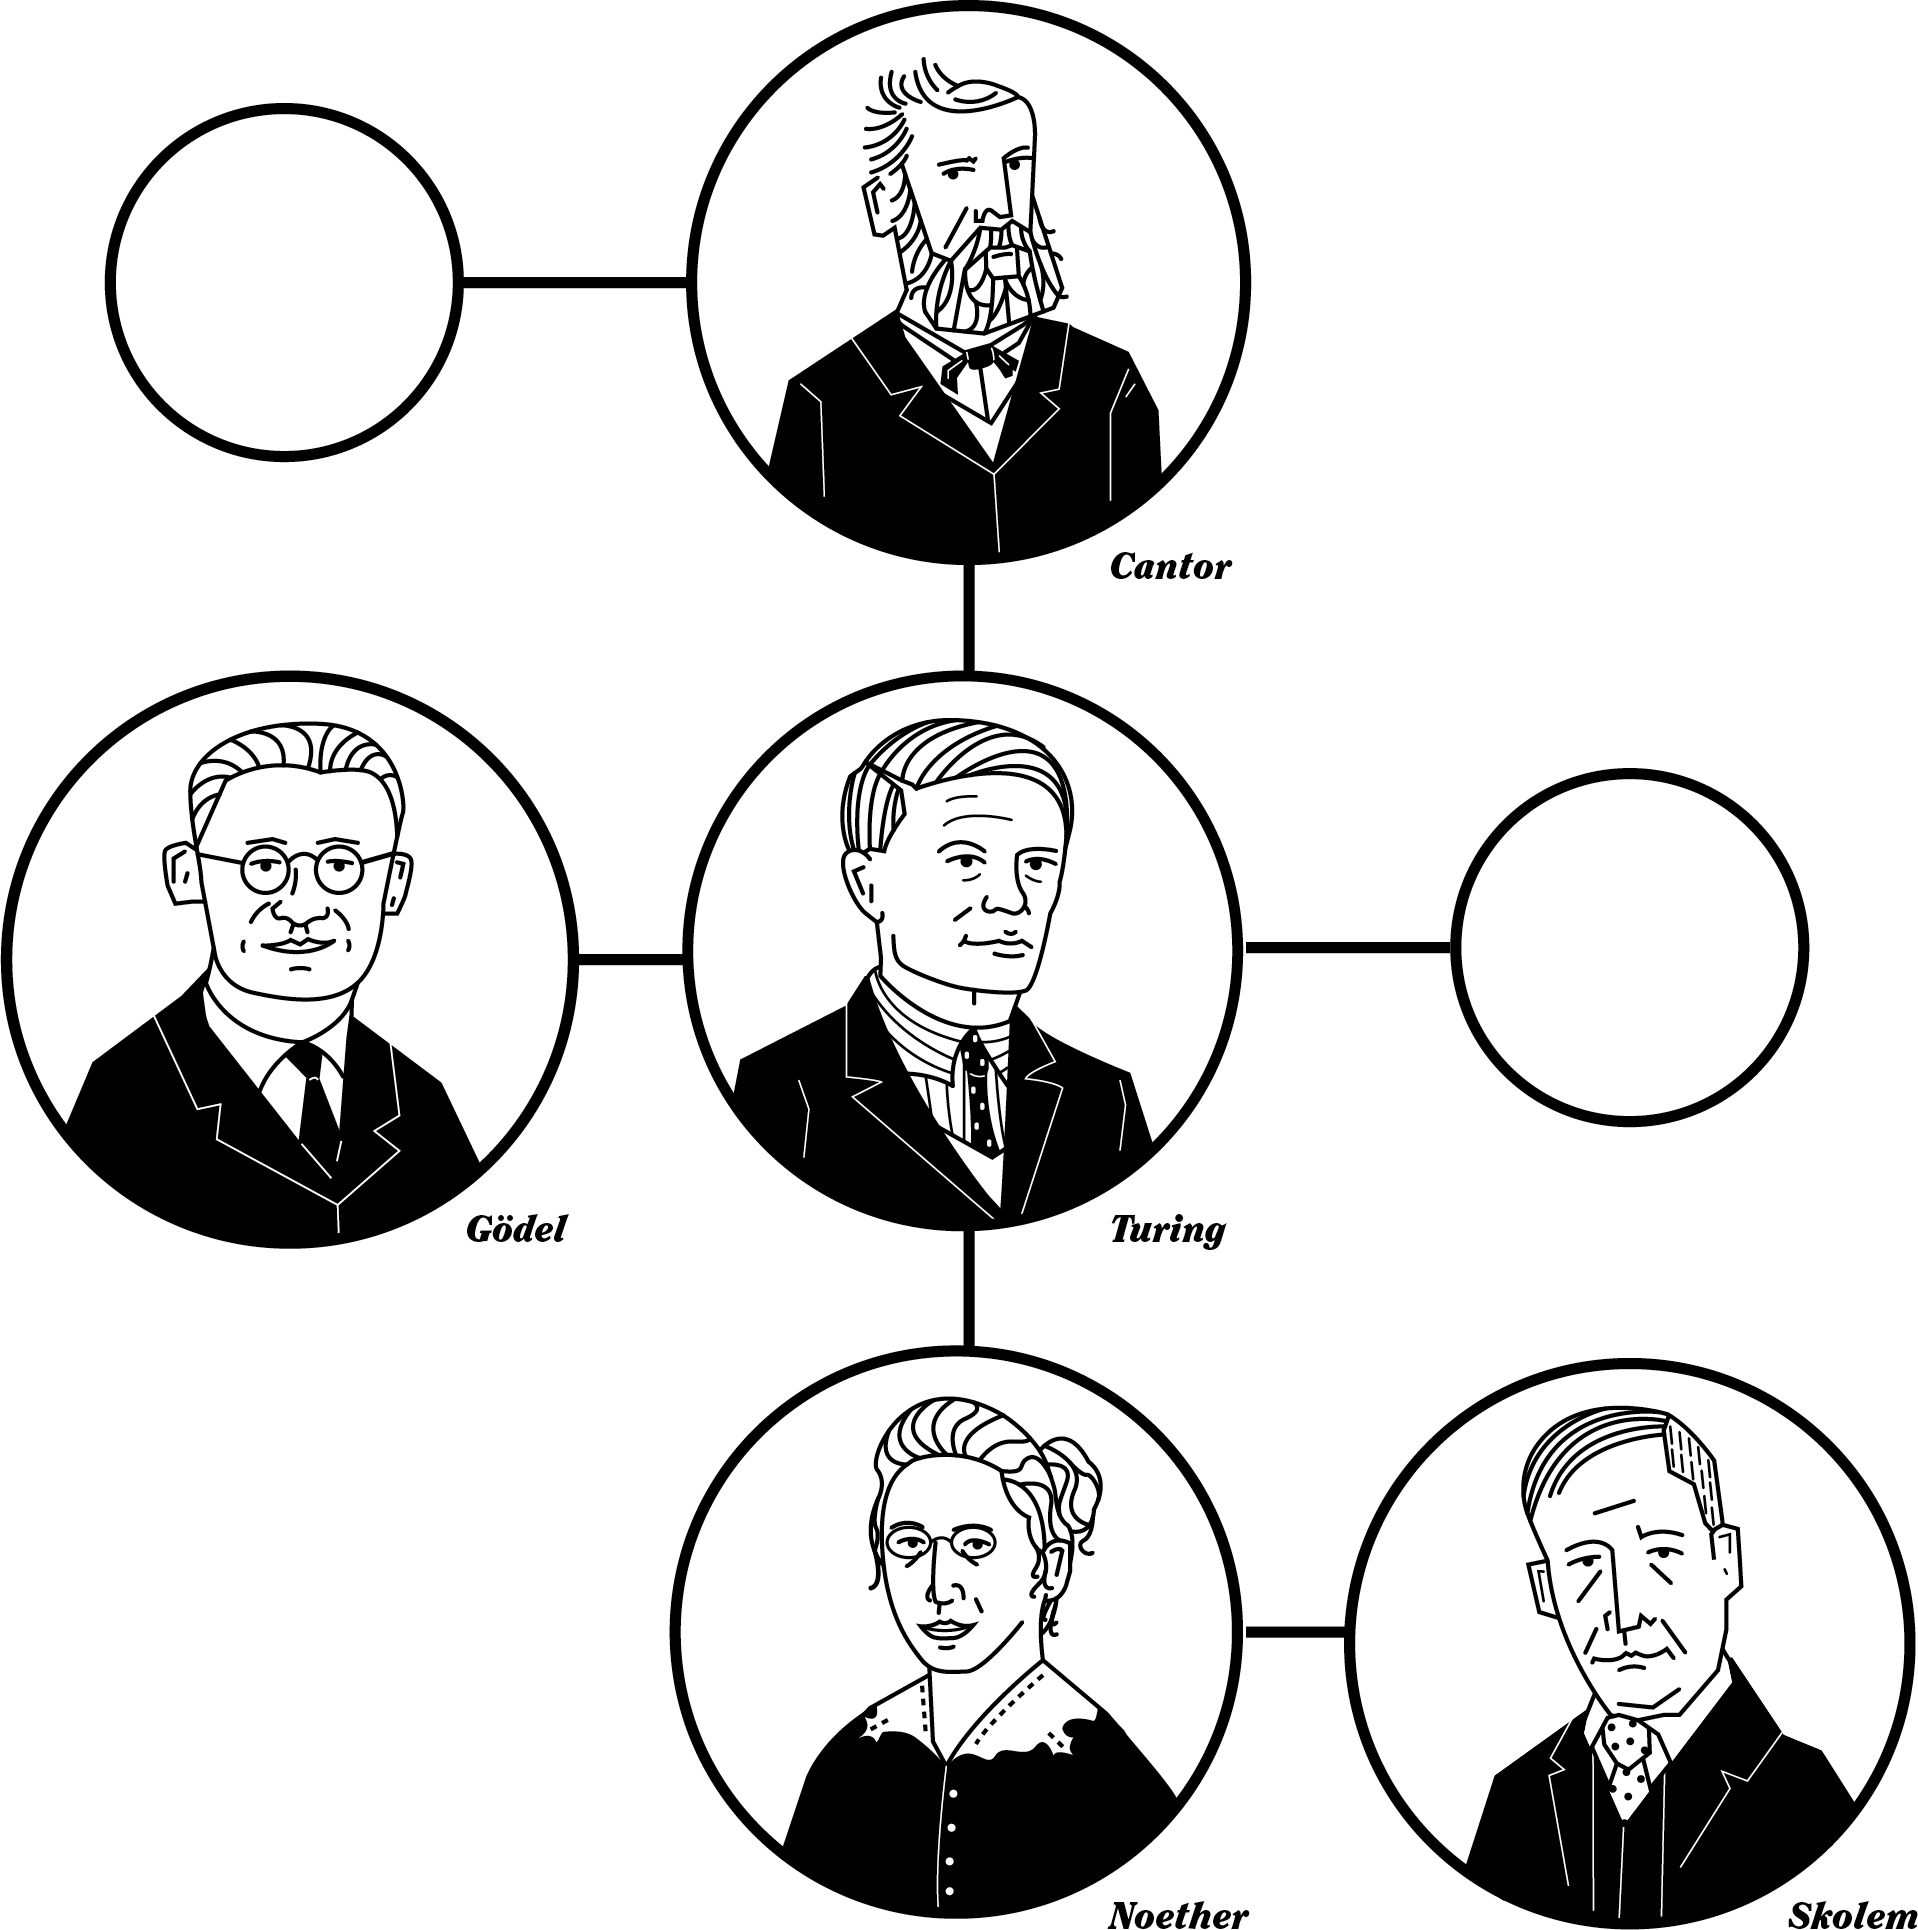
\includegraphics[width=.8\spinepos]{illustrations/Cover}

    \par\noindent
    \vskip 1.5cm
    \noindent
\includegraphics[width=1cm]{assets/cc.pdf}
\includegraphics[width=1cm]{assets/by.pdf}
\includegraphics[width=1cm]{assets/remix.pdf}
\normalfont\fontsize{16pt}{0pt}\selectfont\bfseries\sffamily%
\hfill Fall 2017% \textit{bis}
\end{minipage}
\hfil
  \end{textblock*}

% make back cover
\begin{textblock*}{\spinepos}(0pt,0pt)
  \noindent\hspace{1.5cm}
  \begin{minipage}[b][\coverheight][b]{.85\spinepos}
\begin{minipage}[b]{1cm}
\includegraphics[width=.8cm]{assets/cc.pdf}
\includegraphics[width=.8cm]{assets/by.pdf}
\includegraphics[width=.8cm]{assets/remix.pdf}
\end{minipage}
\hspace{.3cm}
\begin{minipage}[b]{4.7cm}
  \fontsize{11pt}{1.4em}\selectfont\textit{Sets, Logic, Computation}
by Richard Zach is licensed under a Creative Commons Attribution 4.0
International License.
\end{minipage}
\hfill
\vspace*{2cm}
  \end{minipage}
  \hfill
\end{textblock*}

\end{document}
